\chapter{Dữ liệu Tick}
\label{ch:M3L3}

% Lesson: Tick Data

\section*{Lesson Notes}

MODULE 3 | BÀI 3

{\small
\begin{longtable}{>{\raggedright\arraybackslash}p{0.213\linewidth}>{\raggedright\arraybackslash}p{0.727\linewidth}}
\toprule
\textbf{Thời gian đọc} & 6 giờ \\
\addlinespace[2pt]
\textbf{Kiến thức nền tảng} & Chuỗi thời gian tài chính, pandas, matplotlib \\
\addlinespace[2pt]
\textbf{Từ khóa} & Dữ liệu tick, dữ liệu Cấp 1 (Level 1), TOB, độ nhọn (kurtosis), mất cân bằng dòng lệnh (order flow imbalance), resample, giao dịch (trade), báo giá (quote) \\
\addlinespace[2pt]
\bottomrule
\end{longtable}
}

\emph{Trong bài học này, chúng ta sẽ làm việc trực tiếp với dữ liệu tick, dạng thông tin thị trường tài chính chi tiết nhất. Chúng ta bắt đầu từ những điều cơ bản: dữ liệu tick là gì, vì sao nó được gọi như vậy, và vì sao nó quan trọng đến thế. Sau đó, chúng ta sẽ trực tiếp làm việc với các tập dữ liệu thực, học cách làm sạch và xử lý loại thông tin thị trường có độ phân giải cao này.
Vì sao điều này quan trọng? Bởi vì các thị trường tài chính ngày càng tự động hóa, việc hiểu dữ liệu tần suất cao đang trở nên thiết yếu đối với bất kỳ ai nghiêm túc với tài chính định lượng hoặc giao dịch thuật toán. Chúng ta sẽ làm việc với dữ liệu tick thực tế từ các sàn giao dịch tiền mã hóa và thị trường chứng khoán. Dữ liệu này lộn xộn và nhiều thách thức, nhưng đó chính là một phần của quy trình làm việc này. Đến cuối bài học, bạn sẽ có kinh nghiệm thực tế trong việc xử lý loại dữ liệu này, từ khâu làm sạch cho đến việc tạo ra các biểu đồ tổng hợp theo thời gian mà có lẽ bạn quen thuộc hơn.}

\section{Dữ liệu Tick là gì?}

Trong các thị trường tài chính, dữ liệu là phương tiện thúc đẩy việc ra quyết định và các chiến lược giao dịch. Trong số các loại dữ liệu thị trường hiện có, dữ liệu tick là loại chi tiết và toàn diện nhất. Dữ liệu tick là bản ghi chi tiết nhất về hoạt động giao dịch, bao gồm từng giao dịch đơn lẻ xảy ra trên một sàn. Nó gồm giá, khối lượng và mốc thời gian của mỗi giao dịch (và tùy sàn giao dịch hoặc nhà cung cấp dữ liệu, có thể có thêm các cột khác), cho phép những người tham gia thị trường phân tích động lực thị trường ở mức cơ bản nhất.

Nhưng tại sao ta dùng thuật ngữ ``tick''?

Giá của một tài sản dường như là một biến liên tục. Thật vậy, khi quan sát đồ thị của một tài sản, người ta có thể suy ra rằng giá có thể nhận bất kỳ giá trị nào giữa điểm giá A và B. Nhưng thực tế không phải vậy. Giá là một biến rời rạc, dịch chuyển theo các bước nhảy là bội của một đơn vị nhỏ gọi là ``tick''.

Về bản chất, từ ``tick'' chỉ mức dịch chuyển giá nhỏ nhất của một tài sản (cổ phiếu, hàng hóa hoặc hợp đồng tương lai), và nó có thể khác nhau đối với cùng một tài sản giữa các sàn giao dịch và các nhà môi giới (Harris). Ví dụ, nếu kích thước tick (tick size) của một cổ phiếu là \$0.01 và giá cổ phiếu là \$100, thì giá chỉ có thể là $\$100 + \lambda \cdot 0.01$ với $\lambda \in \mathbb{Z}$. Ta có thể có mức giá \$100.01 hoặc \$100.15 nhưng không bao giờ có \$100.005.

Về mặt lịch sử, thuật ngữ ``tick'' bắt nguồn từ âm thanh của các máy điện báo chứng khoán (stock ticker) thời kỳ đầu vào cuối thế kỷ 19, vốn in giá cổ phiếu lên một băng giấy (ticker tape).

\textbf{Băng giấy Ticker của Cuộc Khủng hoảng năm 1929}

\begin{figure}[H]
\centering
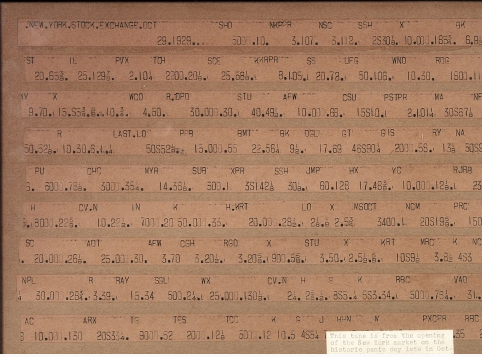
\includegraphics[width=\linewidth,height=0.4\textheight,keepaspectratio]{gfx/m3l3_notes_fig0_crash1929_ticker_tape.png}
\end{figure}

\emph{Khi các máy điện báo chứng khoán ghi lại giá cổ phiếu, mỗi giao dịch đều đi kèm một tiếng ``tích''.}

Nguồn: Museum of American Finance. ``Crash of 1929 Ticker Tape.'' \url{https://www.moaf.org/publications-collections/museum-collection/objects/crash-1929-ticker-tape}

``Dữ liệu tick'' được biết đến qua nhiều tên gọi, mỗi tên làm lộ ra một đặc điểm quan trọng của nó:

\begin{itemize}
  \item \textbf{Dữ liệu từng tick (tick-by-tick data)}: Mỗi điểm dữ liệu là một tick.
  \item \textbf{Dữ liệu tần suất (siêu) cao (High-Frequency data)}: Tần suất của các tick và khối lượng giao dịch rất cao, đặc biệt trong các thị trường có tính thanh khoản cao.
  \item \textbf{Giao dịch (Trades)}: Mỗi tick đại diện cho một giao dịch.
  \item \textbf{Giao dịch khớp lệnh (Transactions)}: Mỗi giao dịch là một giao dịch khớp giữa hai bên.
  \item \textbf{Dữ liệu thời gian thực (Real-time data)}: Dữ liệu này có thể được phân phối theo thời gian thực với độ trễ tối thiểu.
\end{itemize}

Dữ liệu tick không chỉ bao gồm dữ liệu giao dịch mà còn có thể bao gồm dữ liệu báo giá (quote). Dữ liệu này được gọi là sổ lệnh giới hạn (limit order book). Vì vậy, nếu một nhà tạo lập thị trường (market maker) tăng KHỐI LƯỢNG mà họ sẵn sàng mua và đặt một lệnh ở phía giá chào mua (bid), sẽ có thêm một quan sát làm thay đổi kích thước giá chào mua.

Tương tự, nếu một nhà tạo lập thị trường nâng giá chào mua (mức giá mà họ sẵn sàng mua), đó cũng sẽ là một quan sát bổ sung. Ngay cả khi không có giao dịch nào, dữ liệu sổ lệnh giới hạn vẫn là một nguồn thông tin phong phú chứa đựng ý định của những người tham gia. Như bạn sẽ thấy trong Hình 3.7, các ý định (giá chào mua mới, giá chào bán mới, hủy lệnh, v.v.) thay đổi nhanh hơn các hành động (các giao dịch thực tế) của những người tham gia.

Đến lúc này, có thể bạn đã có ít nhiều tiếp xúc với dữ liệu tài chính. Hầu hết mọi người đã từng thấy biểu đồ nến (candlestick) và biểu đồ giá với khoảng thời gian cố định trên trục $x$. Có những ứng dụng trực tuyến như TradingView hay Yahoo Finance và nhiều sàn giao dịch trực tuyến nơi người ta có thể vẽ đồ thị cổ phiếu mình chọn ở bất kỳ khoảng thời gian cố định nào và thậm chí dùng các chỉ báo yêu thích. Về bản chất, những gì bạn thấy là một tập dữ liệu có cấu trúc được tạo ra sau khi một số người hoặc đoạn mã chạy ngầm đã thu thập dữ liệu tick và tạo ra các thanh thời gian (time bar).

Mục đích của bài học này không chỉ là giới thiệu dữ liệu tick cho sinh viên, cho thấy dữ liệu trông như thế nào khi mới được tạo ra, mà còn hướng dẫn bạn tạo và vẽ các tập dữ liệu có cấu trúc mà bạn đã sử dụng từ trước đến nay. Nhờ vậy, chúng ta sẽ chuyển từ dữ liệu ở khâu sản xuất (dữ liệu tick) sang các tập dữ liệu sẵn sàng cho tiêu thụ, tương tự những tập sẽ được dùng trong các môn học sau cho mô hình hóa và phân tích.

Cần thấy rõ rằng dữ liệu tick (và hơn thế nữa là sổ lệnh tần suất cao) bao gồm dữ liệu chi tiết nhất mà bạn có thể tìm thấy. Nếu nghĩ hơi ngây thơ, người ta có thể nói rằng đây là toàn bộ dữ liệu được tạo ra khi giao dịch diễn ra, và do đó ta có thể kỳ vọng nó chứa mọi thông tin có thể có. Mặt khác, cũng có người có thể lập luận rằng còn nhiều yếu tố bên ngoài như xu hướng kinh tế vĩ mô, tâm lý thị trường, quy định pháp lý, tin tức, v.v. Tuy nhiên, nếu bạn tin vào giả thuyết thị trường hiệu quả, thì bạn nên kỳ vọng rằng bất kỳ yếu tố bên ngoài nào cũng sẽ được phản ánh vào giá ngay lập tức. Như vậy, thông tin bên ngoài trở thành một phần của giá và của dữ liệu giao dịch nói chung ngay khi nó được biết đến.

Vì dữ liệu tick có thể được phân phối theo thời gian thực, những nhà giao dịch phân tích dữ liệu này thay vì các thanh thời gian theo phút, giờ hoặc ngày (vốn lần lượt gộp thông tin trong một phút, một giờ hoặc một ngày) sẽ có thể trích xuất thông tin trước những người tham gia còn lại. Tuy nhiên, những nhà giao dịch này phải đối mặt với một nhiệm vụ rất khó: tách thông tin khỏi nhiễu.

\section{Các Ví dụ về Dữ liệu Tick}

Cho mục đích của bài học này, chúng tôi chọn ba tập dữ liệu tần suất cao khác nhau. Hai trong số đó gồm dữ liệu giao dịch từng tick, và tập thứ ba là dữ liệu Level 1 trộn với các giao dịch. Việc chọn các tài sản là ngẫu nhiên và chủ yếu bị ảnh hưởng bởi tính sẵn có của dữ liệu đó. Hầu như luôn luôn, dữ liệu tần suất cao không được cung cấp miễn phí mà khá đắt đỏ. Điều này là bình thường nếu xét đến lượng dữ liệu khổng lồ được tạo ra mỗi ngày và những khó khăn kỹ thuật trong việc lưu trữ và phân phối nó.

Vì lý do này, chúng ta sẽ khám phá:

1.) Các giao dịch từng tick BTC/USDT tải từ sàn Kraken: \url{https://support.kraken.com/hc/en-us/articles/360047543791-Downloadable-historical-market-data-time-and-sales-}

2.) Các giao dịch từng tick RVN/USDT tải từ sàn Binance: \url{https://data.binance.vision/}

3.) Dữ liệu Level 1 AGLJ/ZAR kèm các giao dịch, tải từ: \url{https://data.mendeley.com/datasets/4rrk89c3b2/2}

Do các hạn chế của máy ảo (VM), chỉ một phần rất nhỏ của dữ liệu trên được lấy mẫu cho mục đích giảng dạy. Nhưng bạn được khuyến khích tải các tập dữ liệu từng tick lớn về máy cục bộ để trực tiếp đối mặt với những khó khăn kỹ thuật khi xử lý dữ liệu lớn.

Dữ liệu giao dịch từng tick gồm các cột sau:

\begin{itemize}
  \item Symbol: mã định danh duy nhất của công cụ tài chính.
  \item Timestamp: thời điểm chính xác khi giao dịch được ghi nhận (độ chi tiết từ giây đến nano giây).
  \item Price: giá khớp của giao dịch.
  \item Volume: số đơn vị được giao dịch.
  \item Trade Direction (tùy chọn): cho biết giao dịch do bên mua hay bên bán khởi tạo.
\end{itemize}

Khía cạnh quan trọng nhất của dữ liệu tick, tức độ chi tiết (granularity), cho phép ta thực hiện:

\begin{itemize}
  \item Nghiên cứu độ biến động trong ngày.
  \item Hiểu quá trình hình thành giá một cách thấu đáo hơn.
  \item Kiểm định lùi (backtesting) các chiến lược giao dịch tần suất cao (HF).
  \item Đánh giá tác động thị trường để xác định việc mở rộng quy mô một chiến lược.
  \item Phân tích chi phí giao dịch của một chiến lược.
  \item Khám phá các chiến lược thực thi lệnh.
  \item Phát hiện thao túng thị trường (có thể được các cơ quan quản lý sử dụng).
  \item Tổng hợp thành các thanh theo thời gian hoặc theo khối lượng.
\end{itemize}

\begin{lstlisting}[language=Python,escapeinside={(*@}{@*)}]
import numpy as np
import pandas as pd
import matplotlib.pyplot as plt
import seaborn as sns
sns.set()
\end{lstlisting}

\begin{lstlisting}[language=Python,escapeinside={(*@}{@*)}]
# (*@Tải@*) (*@dữ@*) (*@liệu@*), (*@tập@*) (*@dữ@*) (*@liệu@*) (1) - BTC/USD (*@từ@*) Kraken
btc_usdt = pd.read_csv("XBTUSDT.csv", names=['UNIX_time', 'price', 'volume'])
btc_usdt.head()
\end{lstlisting}

\begin{lstlisting}[escapeinside={(*@}{@*)}]
    UNIX_time    price    volume
0  1688169604  30474.1  0.018800
1  1688169604  30474.8  0.000103
2  1688169604  30476.5  0.014997
3  1688169656  30483.5  0.000614
4  1688170008  30479.0  0.000328
\end{lstlisting}

Tập dữ liệu trên là một ví dụ về tập dữ liệu giao dịch từng tick, và nó gồm tất cả các giao dịch xảy ra trong một khoảng thời gian xác định. Điều đầu tiên bạn nhận thấy là cột UNIX\_time, nó không giống thời gian hay ngày tháng chút nào! Mốc thời gian này được gọi là ``thời gian UNIX'' (UNIX time), và nó đếm số đơn vị thời gian (giây, mili giây, micro giây và nano giây) tính từ 00:00:00 UTC ngày 1 tháng 1 năm 1970 cho đến nay.

Cách biểu diễn thời gian này mang lại:

\begin{itemize}
  \item Tính chuẩn hóa: biểu diễn thời gian phổ quát.
  \item Tính đơn giản: nó chỉ là một số nguyên duy nhất.
  \item Hiệu quả: các phép tính đơn giản và hiệu quả về mặt tính toán.
\end{itemize}

Các mốc thời gian Unix (Unix Timestamps) có thể được biểu diễn với các mức độ chính xác khác nhau:

\begin{itemize}
  \item 10 chữ số: Biểu diễn giây (ví dụ: 1688169604).
  \item 13 chữ số: Bao gồm mili giây (ví dụ: 1688169604123).
  \item 16 chữ số: Bao gồm micro giây (ví dụ: 1688169604123456).
  \item 19 chữ số: Bao gồm nano giây (ví dụ: 1688169604123456789).
\end{itemize}

Bạn cũng có thể xem trang web này: \url{https://unixtime.org/}.

Trong tập dữ liệu (1), ta đếm được 10 chữ số ở cột UNIX\_time. Do đó, độ chính xác được tính bằng giây, và đây là điều duy nhất ta cần biết để chuyển đổi thời gian Unix thành ngày giờ dễ đọc.

\begin{lstlisting}[language=Python,escapeinside={(*@}{@*)}]
# (*@Chuyển@*) (*@mốc@*) (*@thời@*) (*@gian@*) (*@UNIX@*) (*@thành@*) (*@ngày@*) (*@giờ@*) (*@dễ@*) (*@đọc@*). (*@Kiểm@*) (*@tra@*) (*@đối@*) (*@số@*) unit='s' (*@để@*) (*@đảm@*) (*@bảo@*) (*@mốc@*) (*@thời@*) (*@gian@*) (*@tính@*) (*@bằng@*) (*@giây@*).
btc_usdt['timestamp'] = pd.to_datetime(btc_usdt['UNIX_time'], unit='s')
btc_usdt.set_index('timestamp', inplace=True) # (*@Đặt@*) (*@timestamp@*) (*@làm@*) (*@chỉ@*) (*@mục@*)
btc_usdt.head()
\end{lstlisting}

\begin{lstlisting}[escapeinside={(*@}{@*)}]
                      UNIX_time    price    volume
timestamp                                         
2023-07-01 00:00:04  1688169604  30474.1  0.018800
2023-07-01 00:00:04  1688169604  30474.8  0.000103
2023-07-01 00:00:04  1688169604  30476.5  0.014997
2023-07-01 00:00:56  1688169656  30483.5  0.000614
2023-07-01 00:06:48  1688170008  30479.0  0.000328
\end{lstlisting}

\section{Trực quan hóa Dữ liệu Giao dịch Tick}

Bây giờ, hãy xem xét tập dữ liệu của chúng ta bằng hình ảnh. Việc trực quan hóa dữ liệu tick đặt ra những thách thức đặc thù do độ phân giải cực cao của nó. Hãy xét phép so sánh sau: hình dung bạn có một bức ảnh độ phân giải siêu cao được hiển thị trên một màn hình nhỏ hoặc được xem từ xa. Phần lớn chi tiết bị mất đi, và bạn có thể tự hỏi giá trị của độ phân giải cao như vậy là gì. Tương tự, khi vẽ dữ liệu tick, ta có nguy cơ che khuất các mẫu hình quan trọng nếu chỉ đơn giản vẽ mọi điểm. Mấu chốt là tìm những cách biểu diễn dữ liệu tần suất cao này sao cho làm lộ ra các mẫu hình và đặc điểm vốn có của nó mà không làm người xem bị choáng ngợp. Trong mục này, dữ liệu của chúng ta lấy từ ``TRTH JSE AGLJ.J Intraday Transaction Test Data'' của Gebbie và Nonyane và từ các tập dữ liệu được nhắc đến ở mục 2.

\begin{lstlisting}[language=Python,escapeinside={(*@}{@*)}]
#(*@Hình@*) 3.1
fig, ax = plt.subplots(figsize=(12, 5))
ax.scatter(btc_usdt.index, btc_usdt['price'], s = 0.001, alpha=0.4)
ax.set_ylabel('Price')
ax.set_title('BTC/USDT Price')
ax.set_ylim(20000, 32000)

custom_legend = plt.Line2D([0], [0], linestyle="none", marker='o', color='b', markersize=3, alpha = 0.7, label='Price') # (*@Tạo@*) (*@chú@*) (*@giải@*) (*@tùy@*) (*@chỉnh@*)
ax.legend(handles=[custom_legend], loc='upper right')

ax2 = ax.twinx() # (*@Tạo@*) (*@trục@*) (*@y@*) (*@thứ@*) (*@hai@*)
ax2.plot(btc_usdt.index, btc_usdt['volume'].rolling(10000).sum(), color='red', label='Volume: Rolling sum', alpha=0.3)
ax2.set_ylabel('Volume: Rolling sum')
ax2.set_ylim(200, 2300)

ax3 = ax.twinx() # (*@Tạo@*) (*@trục@*) (*@y@*) (*@thứ@*) (*@ba@*)
ax3.plot(btc_usdt.index, btc_usdt['volume'], color='purple', label='Volume', alpha=0.3)
ax3.set_ylabel('Volume')
ax3.set_ylim(0, 40)
ax3.spines['right'].set_position(('outward', 60))

fig.legend(bbox_to_anchor=(0.5,0.56)) # (*@Điều@*) (*@chỉnh@*) (*@vị@*) (*@trí@*) (*@chú@*) (*@giải@*)
plt.show()
\end{lstlisting}

\begin{figure}[H]
\centering
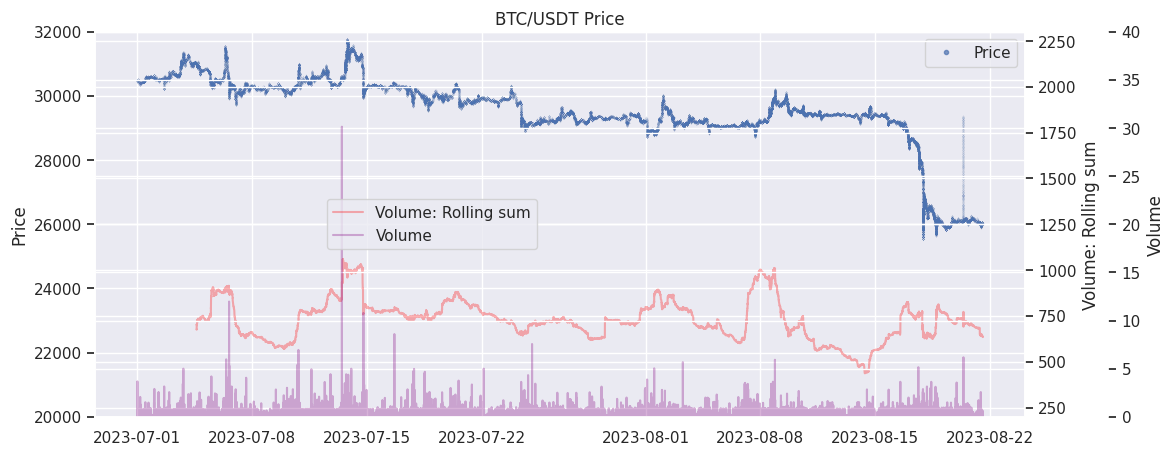
\includegraphics[width=\linewidth,height=0.6\textheight,keepaspectratio]{gfx/m3l3_notes_fig1_btcusdt_price_volume.png}
\par\smallskip{\small \textbf{Hình 3.1:} Giá BTC/USDT (biểu đồ phân tán) cùng khối lượng và tổng khối lượng trượt (rolling sum) trên các trục $y$ thứ hai và thứ ba}
\end{figure}

Cần lưu ý rằng các tập dữ liệu (1) và (2) được lấy trực tiếp từ các sàn giao dịch nơi chúng được tạo ra; do đó, ta kỳ vọng không có đầu vào bị thiếu. Điều đó không có nghĩa là dữ liệu không có lỗi!

Hãy khám phá tập dữ liệu của chúng ta:

\begin{lstlisting}[language=Python,escapeinside={(*@}{@*)}]
between_trades_interval = btc_usdt['UNIX_time'].diff().dropna() # (*@Tính@*) (*@thời@*) (*@lượng@*) (*@giữa@*) (*@các@*) (*@giao@*) (*@dịch@*)
print("Summary Statistics \n\n", between_trades_interval.describe(), "\n\n") # (*@Lấy@*) (*@thống@*) (*@kê@*) (*@tóm@*) (*@tắt@*) (*@của@*) (*@thời@*) (*@lượng@*) (*@giao@*) (*@dịch@*)
print("10 Largest trade durations \n\n", between_trades_interval.sort_values(ascending=False).head(10)) # (*@Lấy@*) 10 (*@khoảng@*) (*@thời@*) (*@gian@*) (*@lớn@*) (*@nhất@*) (*@giữa@*) (*@các@*) (*@giao@*) (*@dịch@*)
\end{lstlisting}

\begin{lstlisting}[escapeinside={(*@}{@*)}]
Summary Statistics 

 count    185042.000000
mean         24.072584
std          61.776399
min           0.000000
25%           0.000000
50%           0.000000
75%          18.000000
max        2195.000000
Name: UNIX_time, dtype: float64 


10 Largest trade durations 

 timestamp
2023-08-01 15:41:45    2195.0
2023-07-12 09:19:13    2001.0
2023-08-17 10:30:32    1809.0
2023-08-18 15:05:14    1576.0
2023-07-23 07:29:23    1281.0
2023-07-23 02:13:51    1244.0
2023-08-06 03:40:46    1224.0
2023-07-20 23:44:23    1125.0
2023-07-16 03:52:08    1113.0
2023-07-19 05:28:45    1100.0
Name: UNIX_time, dtype: float64
\end{lstlisting}

Xét từ các kết quả trên (thời lượng giao dịch cao), cặp BTC/USDT trong mẫu cụ thể này có vẻ kém thanh khoản. Nhưng ta biết rằng tính thanh khoản có thể thay đổi rất lớn theo thời gian và mẫu này có thể không đại diện cho tính thanh khoản của cặp này trên sàn này. Để rút ra kết luận vững chắc hơn, ta cần phân tích một tập dữ liệu lớn hơn, trải dài qua các giai đoạn và điều kiện thị trường khác nhau.

Hãy kiểm tra phân phối của khối lượng, lợi suất đơn giản và các khoảng thời gian giữa các giao dịch.

\begin{lstlisting}[language=Python,escapeinside={(*@}{@*)}]
#(*@Hình@*) 3.2
fig, (ax1, ax2, ax3) = plt.subplots(1, 3, figsize=(15, 4))
ax1.hist(between_trades_interval, bins=100, color='skyblue', edgecolor='black', linewidth=1.2)
ax1.set_title("Time between trades")
ax2.hist(btc_usdt['price'].pct_change().dropna(), bins=100, color='white', edgecolor='black', linewidth=1.2)
ax2.set_title("Simple Returns")
ax3.hist(btc_usdt['volume'], bins=100, color='green', edgecolor='black', linewidth=1.2)
ax3.set_title("Volume")
plt.show()
\end{lstlisting}

\begin{figure}[H]
\centering
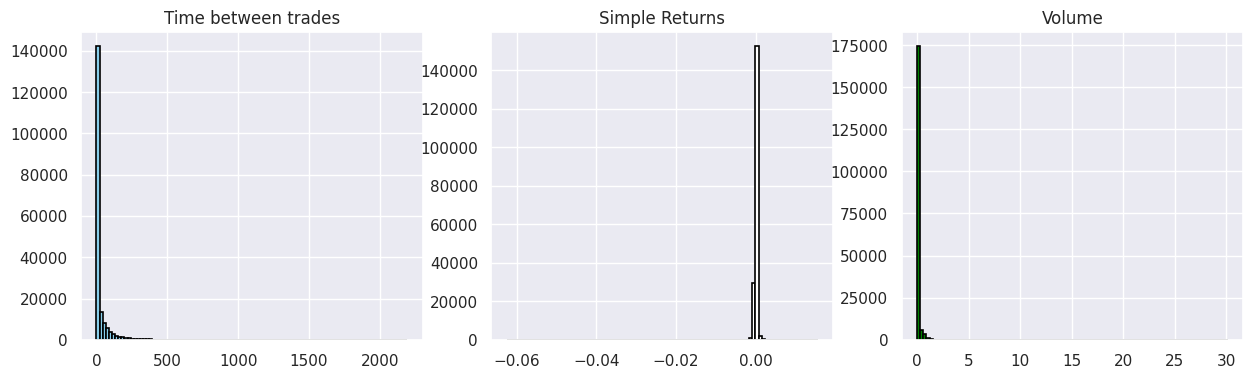
\includegraphics[width=\linewidth,height=0.6\textheight,keepaspectratio]{gfx/m3l3_notes_fig2_raw_tick_histograms.png}
\par\smallskip{\small \textbf{Hình 3.2:} Histogram của thời gian giữa các giao dịch, lợi suất đơn giản và khối lượng của dữ liệu tick BTC/USDT gốc}
\end{figure}

Các kết quả trên gợi ý ba sự thật quan trọng:

\begin{itemize}
  \item Có nhiều giao dịch xảy ra trong cùng một giây. Những giao dịch này có thể là một giao dịch duy nhất bị chia thành nhiều giao dịch tại thời điểm thực thi do khối lượng ở mức giá chào mua hoặc giá chào bán tốt nhất không đủ để đáp ứng khối lượng giao dịch tại thời điểm đó. Những giao dịch này được gọi là \textbf{giao dịch bị chia nhỏ (split transactions)}.
  \item Có nhiều giao dịch không làm giá thay đổi.
  \item Rất nhiều giao dịch dường như có khối lượng rất thấp.
\end{itemize}

\begin{lstlisting}[language=Python,escapeinside={(*@}{@*)}]
boolean_array_is_duplicate = btc_usdt['UNIX_time'].duplicated(keep=False) # (*@Kiểm@*) (*@tra@*) (*@các@*) (*@bản@*) (*@trùng@*) (*@lặp@*)
sum_of_duplicates = boolean_array_is_duplicate.sum() # (*@Tính@*) (*@tổng@*) (*@các@*) (*@bản@*) (*@trùng@*) (*@lặp@*)
print("The number of trades that occured at the same second with at least one more trade, is: ",sum_of_duplicates)
print("The percentage of these trades to the number of all trades, is: ",round(sum_of_duplicates / len(btc_usdt) * 100, 2), "%")
print("The percentage of the volume of these trades to the entire volume, is: ",round(((boolean_array_is_duplicate * btc_usdt['volume']).sum() / btc_usdt['volume'].sum() )* 100, 2), "%")
\end{lstlisting}

\begin{lstlisting}[escapeinside={(*@}{@*)}]
The number of trades that occured at the same second with at least one more trade, is:  126239
The percentage of these trades to the number of all trades, is:  68.22 %
The percentage of the volume of these trades to the entire volume, is:  91.13 %
\end{lstlisting}

Chúng ta sẽ giả định rằng những giao dịch này là các giao dịch bị chia nhỏ. Sau một vài phép tổng hợp đơn giản, các histogram vẽ ở trên trông rất khác:

\begin{lstlisting}[language=Python,escapeinside={(*@}{@*)}]
# (*@Hình@*) 3.3
aggr_dataset_1 = pd.DataFrame()
aggr_dataset_1['UNIX_time'] = btc_usdt['UNIX_time'].groupby(btc_usdt['UNIX_time']).first() # (*@Nhóm@*) (*@mốc@*) (*@thời@*) (*@gian@*) (*@UNIX@*) (*@theo@*) (*@mốc@*) (*@thời@*) (*@gian@*) (*@đầu@*) (*@tiên@*)
aggr_dataset_1['volume'] = btc_usdt['volume'].groupby(btc_usdt['UNIX_time']).sum() # (*@Tổng@*) (*@hợp@*) (*@khối@*) (*@lượng@*) (*@theo@*) (*@mốc@*) (*@thời@*) (*@gian@*) (*@UNIX@*)
aggr_dataset_1['price'] = (btc_usdt['price'] * btc_usdt['volume']).groupby(btc_usdt['UNIX_time']).sum() / aggr_dataset_1['volume'] # (*@Giá@*) (*@cuối@*) (*@cùng@*) (*@là@*) VWAP (*@của@*) (*@giao@*) (*@dịch@*) (*@bị@*) (*@chia@*) (*@nhỏ@*)
aggr_dataset_1.index = btc_usdt.index.drop_duplicates() # (*@Loại@*) (*@bỏ@*) (*@các@*) (*@bản@*) (*@trùng@*) (*@lặp@*) (*@khỏi@*) (*@chỉ@*) (*@mục@*)

fig, (ax1, ax2, ax3) = plt.subplots(1, 3, figsize=(15, 4))
ax1.hist(aggr_dataset_1['UNIX_time'].diff().dropna(), bins=100, color='skyblue', edgecolor='black', linewidth=1.2)
ax1.set_title("Time between trades")
ax2.hist(aggr_dataset_1['price'].pct_change().dropna(),bins=100, color='white', edgecolor='black', linewidth=1.2)
ax2.set_title("Simple Returns")
ax3.hist(aggr_dataset_1['volume'], bins=100, color='green', edgecolor='black', linewidth=1.2)
ax3.set_title("Volume")
plt.show()
\end{lstlisting}

\begin{lstlisting}[escapeinside={(*@}{@*)}]
/tmp/ipykernel_45/2642210345.py:11: FutureWarning: The default fill_method='pad' in Series.pct_change is deprecated and will be removed in a future version. Either fill in any non-leading NA values prior to calling pct_change or specify 'fill_method=None' to not fill NA values.
  ax2.hist(aggr_dataset_1['price'].pct_change().dropna(),bins=100, color='white', edgecolor='black', linewidth=1.2)
\end{lstlisting}

\begin{figure}[H]
\centering
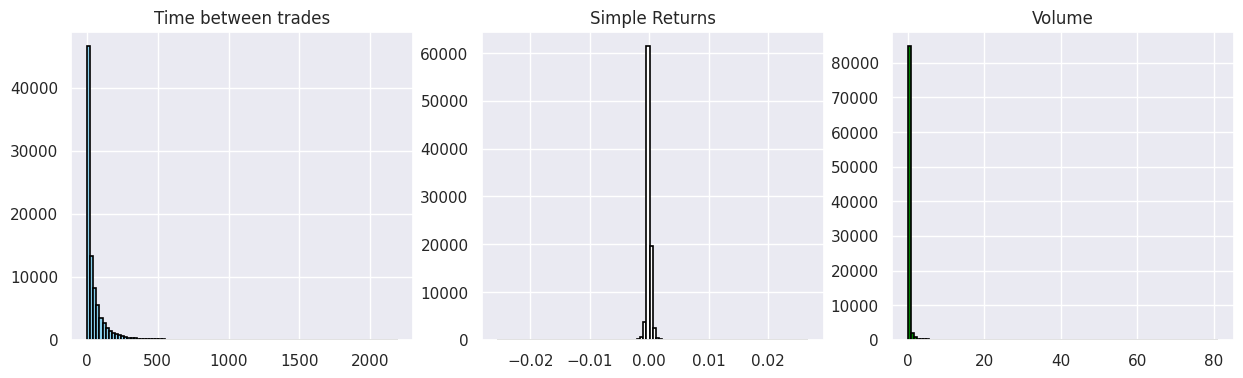
\includegraphics[width=\linewidth,height=0.6\textheight,keepaspectratio]{gfx/m3l3_notes_fig3_aggregated_histograms.png}
\par\smallskip{\small \textbf{Hình 3.3:} Histogram của thời gian giữa các giao dịch, lợi suất đơn giản và khối lượng sau khi tổng hợp các giao dịch bị chia nhỏ}
\end{figure}

Tại thời điểm này, ta có thể tiếp tục quy trình bằng phân tích lợi suất, mất cân bằng dòng lệnh (order flow imbalance, OFI), ước lượng độ biến động, thước đo thanh khoản, v.v. Vì các tập dữ liệu này sẽ được dùng để trình bày dữ liệu tick chứ không phải để phân tích, chúng ta sẽ chuyển sang tập dữ liệu (2), và một quy trình giới thiệu sẽ được trình bày với tập dữ liệu (3).

\section{Bao gồm Hướng Giao dịch}

Hãy xem tập dữ liệu (2), chứa các giao dịch RVN/USDT nhưng có thêm một điều so với tập dữ liệu (1): có một cột bổ sung, ``Trade Direction'', chứa thông tin cho biết nhà giao dịch khởi tạo giao dịch là bên mua hay bên bán. Trong trường hợp của chúng ta, sàn giao dịch lưu một giá trị boolean (True, False) cho mỗi dòng, trả lời câu hỏi \emph{bên mua có phải là nhà tạo lập thị trường (market maker) hay không?}

Như ta biết, mỗi giao dịch phải có một bên mua và một bên bán. Nếu câu trả lời cho câu hỏi trên là đúng (true), thì nhà tạo lập thị trường đã đặt một lệnh chào mua (bid) vào sổ lệnh với ý định mua, và một bên bán đã khởi tạo giao dịch bằng cách khớp (một phần?) lệnh mua đó. Ngược lại, nếu câu trả lời là sai (false), thì nhà tạo lập thị trường là bên bán đã đặt một lệnh chào bán (ask). Trong trường hợp này, bên khởi tạo giao dịch là một bên mua đã khớp lệnh chào bán cụ thể đó.

Mảng boolean bổ sung này là một nguồn thông tin có giá trị.

Chúng ta sẽ bắt đầu bằng việc tải tập dữ liệu (2). Trong nhiều trường hợp, nhà cung cấp dữ liệu hoặc sàn giao dịch sẽ cho phép bạn tải dữ liệu dưới dạng các tệp \texttt{csv}, mỗi tệp chứa dữ liệu của một ngày (hoặc một tuần, hoặc một tháng, hoặc một khoảng thời gian tùy chỉnh). Trong trường hợp của chúng ta, tập dữ liệu (2) gồm bốn tệp theo ngày. Chúng ta sẽ dùng thư viện \texttt{glob} vì sự đơn giản của nó trong việc chọn các tệp cần thiết: \url{https://builtin.com/software-engineering-perspectives/glob-in-python}.

\begin{lstlisting}[language=Python,escapeinside={(*@}{@*)}]
import glob

# (*@Tải@*) (*@dữ@*) (*@liệu@*), (*@tập@*) (*@dữ@*) (*@liệu@*) (2) - RVN/USDT
list_of_files = glob.glob('RVNUSDT*') # (*@Liệt@*) (*@kê@*) (*@các@*) (*@tệp@*) RVNUSDT (*@trong@*) (*@thư@*) (*@mục@*)
column_names = ['id', 'price', 'qty', 'base_qty', 'UNIX_time', 'is_buyer_maker', 'is_best_match'] # (*@Tên@*) (*@các@*) (*@cột@*)
rvn_usdt = pd.concat([pd.read_csv(file, names=column_names) for file in list_of_files], ignore_index=True, axis = 0) # (*@Nối@*) (*@các@*) (*@tệp@*)
rvn_usdt.sort_values('UNIX_time', inplace=True) # (*@Sắp@*) (*@xếp@*) (*@các@*) (*@giá@*) (*@trị@*) (*@theo@*) (*@thời@*) (*@gian@*)
rvn_usdt.head(5)
\end{lstlisting}

\begin{lstlisting}[escapeinside={(*@}{@*)}]
              id    price      qty    base_qty     UNIX_time is_buyer_maker  \
148005  55947315  0.02103  10000.0  210.300000  1.688100e+04            NaN   
148006  54407520  0.02588    424.9   10.996412  1.680307e+12          False   
148007  54407521  0.02588   3313.5   85.753380  1.680307e+12          False   
148008  54407522  0.02588   4172.5  107.984300  1.680307e+12          False   
148011  54407525  0.02589   1105.3   28.616217  1.680307e+12          False   

       is_best_match  
148005           NaN  
148006          True  
148007          True  
148008          True  
148011          True  
\end{lstlisting}

Hãy lùi lại một chút. Tập dữ liệu (2) là một tập dữ liệu giao dịch từng tick, nhưng có số cột gấp đôi so với tập dữ liệu (1). Đến đây cần thấy rõ rằng, tùy nhà cung cấp dữ liệu và/hoặc sàn giao dịch, có thể có thêm các cột ngoài ba cột cơ bản (giá, khối lượng và mốc thời gian). Trong trường hợp của chúng ta, phần bổ sung có ý nghĩa duy nhất so với các cột cơ bản là cột \texttt{is\_buyer\_maker}.

Cột \texttt{base\_qty} biểu diễn khối lượng của tiền tệ cơ sở (loại tiền tệ mà tài sản được giao dịch đối ứng) được giao dịch, cho trước khối lượng tài sản được giao dịch và giá của giao dịch: $\text{base\_qty} = \text{qty} \cdot \text{price}$. Cột \texttt{id} biểu diễn mã định danh của từng giao dịch và có thể dùng để lọc các bản ghi trùng lặp. Cuối cùng, cột \texttt{is\_best\_match} là một mảng boolean cho biết giao dịch có được thực thi tại mức giá tốt nhất có thể, xét theo sổ lệnh tại thời điểm đó, hay không (True hoặc False).

Chúng ta sẽ kiểm tra xem các cột bổ sung có chứa thông tin nào không trước khi loại bỏ chúng để xử lý một tập dữ liệu nhỏ hơn, giúp giảm tải cho bộ nhớ RAM.

\begin{lstlisting}[language=Python,escapeinside={(*@}{@*)}]
print("Number of duplicate entries: ", rvn_usdt['id'].duplicated().sum()) # (*@Kiểm@*) (*@tra@*) (*@các@*) (*@bản@*) (*@trùng@*) (*@lặp@*)
print("Number of entries that were not executed at the best possible price: ",  (~(rvn_usdt['is_best_match'].astype("bool"))).sum()) # (*@Kiểm@*) (*@tra@*) (*@khớp@*) (*@tốt@*) (*@nhất@*)
print("Can the base_qty be derived from the qty and price?: ", np.isclose(rvn_usdt['price'] * rvn_usdt['qty'], rvn_usdt['base_qty'], atol=1e-05).all()) # (*@Kiểm@*) (*@tra@*) (*@xem@*) (*@lượng@*) (*@cơ@*) (*@sở@*) (*@có@*) (*@thể@*) (*@suy@*) (*@ra@*) (*@từ@*) (*@lượng@*) (*@giao@*) (*@dịch@*) (*@hay@*) (*@không@*)
print("Due to the results above, we can drop the columns 'id', 'is_best_match' and 'base_qty' \n\n")

rvn_usdt = rvn_usdt.drop(columns=['id', 'is_best_match', 'base_qty']) # (*@Loại@*) (*@bỏ@*) (*@các@*) (*@cột@*) (*@không@*) (*@cần@*) (*@thiết@*)
rvn_usdt['timestamp'] = pd.to_datetime(rvn_usdt['UNIX_time'], unit='ms') # (*@Chuyển@*) (*@mốc@*) (*@thời@*) (*@gian@*) (*@UNIX@*) (*@thành@*) (*@ngày@*) (*@giờ@*) (*@dễ@*) (*@đọc@*). (*@Kiểm@*) (*@tra@*) (*@đối@*) (*@số@*) unit='ms' (*@để@*) (*@đảm@*) (*@bảo@*) (*@mốc@*) (*@thời@*) (*@gian@*) (*@tính@*) (*@bằng@*) (*@mili@*) (*@giây@*).
rvn_usdt.set_index('timestamp', inplace=True) # (*@Đặt@*) (*@timestamp@*) (*@làm@*) (*@chỉ@*) (*@mục@*)
rvn_usdt.head()
\end{lstlisting}

\begin{lstlisting}[escapeinside={(*@}{@*)}]
Number of duplicate entries:  0
Number of entries that were not executed at the best possible price:  0
Can the base_qty be derived from the qty and price?:  False
Due to the results above, we can drop the columns 'id', 'is_best_match' and 'base_qty' 



                           price      qty     UNIX_time is_buyer_maker
timestamp                                                             
1970-01-01 00:00:16.881  0.02103  10000.0  1.688100e+04            NaN
2023-04-01 00:00:15.745  0.02588    424.9  1.680307e+12          False
2023-04-01 00:00:15.759  0.02588   3313.5  1.680307e+12          False
2023-04-01 00:00:15.759  0.02588   4172.5  1.680307e+12          False
2023-04-01 00:00:15.762  0.02589   1105.3  1.680307e+12          False
\end{lstlisting}

\section{Xử lý Dữ liệu Tick}

Từ đây trở đi, khi nói ``khối lượng mua'' (buying volume) hay ``khối lượng bán'' (selling volume), chúng ta sẽ chỉ khối lượng của các giao dịch mà bên khởi tạo/bên nhận lệnh (taker) lần lượt là bên mua hoặc bên bán. Để hiểu cách sử dụng thông tin bổ sung này, chúng ta sẽ trình bày các thao tác xử lý dữ liệu thiết yếu để tính khối lượng mua và khối lượng bán.

\begin{lstlisting}[language=Python,escapeinside={(*@}{@*)}]
# (*@Hình@*) 3.4
buying_volume = rvn_usdt['qty'] * (~(rvn_usdt['is_buyer_maker'].astype("bool"))) # (*@Một@*) (*@mảng@*) (*@chứa@*) (*@khối@*) (*@lượng@*) (*@mua@*)
selling_volume = rvn_usdt['qty'] * rvn_usdt['is_buyer_maker'].astype("bool") # (*@Một@*) (*@mảng@*) (*@chứa@*) (*@khối@*) (*@lượng@*) (*@bán@*)

print("The buying volume is: ", buying_volume.sum()) # (*@Tính@*) (*@khối@*) (*@lượng@*) (*@mua@*)
print("The selling volume is: ", selling_volume.sum()) # (*@Tính@*) (*@khối@*) (*@lượng@*) (*@bán@*)

fig, (ax1, ax2) = plt.subplots(1, 2, figsize=(15, 4))
ax1.hist(buying_volume, log = True, bins=100, color='skyblue', edgecolor='black', linewidth=1.2)
ax1.set_title("Buying Volume")
ax2.hist(selling_volume, log = True, bins=100, color='green', edgecolor='black', linewidth=1.2)
ax2.set_title("Selling Volume")
plt.show()
\end{lstlisting}

\begin{lstlisting}[escapeinside={(*@}{@*)}]
The buying volume is:  658280433.4000001
The selling volume is:  684682634.6999999
\end{lstlisting}

\begin{figure}[H]
\centering
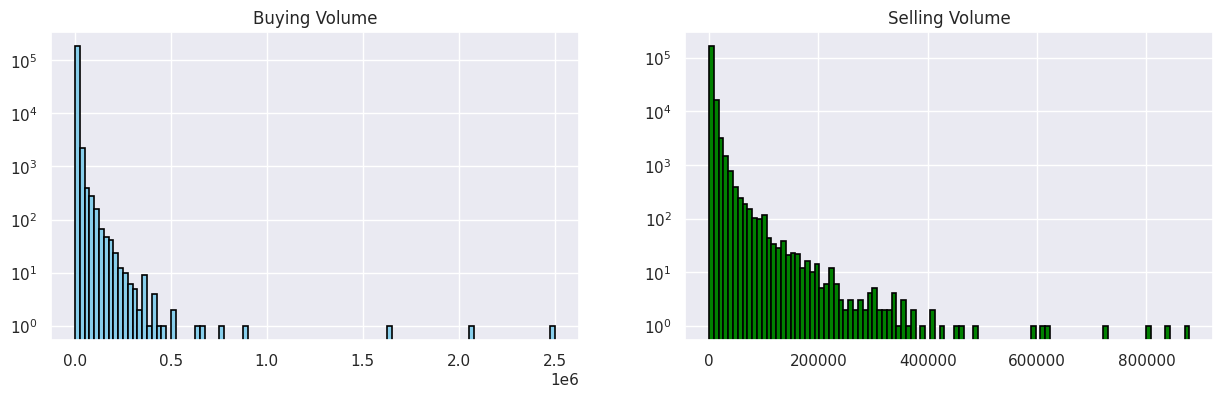
\includegraphics[width=\linewidth,height=0.6\textheight,keepaspectratio]{gfx/m3l3_notes_fig4_buying_selling_volume.png}
\par\smallskip{\small \textbf{Hình 3.4:} Histogram (trục $y$ theo thang log) của khối lượng mua và khối lượng bán của RVN/USDT}
\end{figure}

\textbf{Bài tập 1}

Trong histogram ở trên, chúng ta đã dùng đối số \texttt{log = True} để chuyển trục $y$ sang thang log. Để hiểu vì sao, hãy vẽ các histogram của khối lượng mua và khối lượng bán với \texttt{log = False}. Hơn nữa, hãy phân biệt giữa việc biến đổi trục $y$ cho mục đích trực quan hóa và việc biến đổi chính dữ liệu bằng logarit tự nhiên. Hãy tạo lại hai histogram với \texttt{log = False}, nhưng dùng hàm \texttt{np.log} để biến đổi khối lượng mua và khối lượng bán: \texttt{np.log(buying\_volume[buying\_volume > 1])}. Làm tương tự với các histogram trình bày trong Hình 3.3. Hãy giải thích các khác biệt.

\textbf{Bài tập 2}

Tính kích thước tick (tick size) cho các tập dữ liệu (1) và (2). Hãy giải thích phương pháp của bạn trên diễn đàn.

Bây giờ chúng ta sẽ vẽ khối lượng mua và khối lượng bán theo cách trực quan bắt mắt. Khi vẽ dữ liệu độ phân giải cao, việc thu nhỏ để xem ``bức tranh toàn cảnh'' là vô nghĩa. Ngược lại, chúng ta chọn các đồ thị phóng to hoặc các đồ thị tương tác (plotly, bokeh) nơi ta có thể phóng to theo yêu cầu.

\begin{lstlisting}[language=Python,escapeinside={(*@}{@*)}]
# (*@Hình@*) 3.5
start = rvn_usdt.index[rvn_usdt.index >= "2023-07-01 01:53:15.745"][0]
end   = rvn_usdt.index[rvn_usdt.index <= "2023-07-01 01:54:15.745"][-1]

rvn_usdt_slice = rvn_usdt.loc[start:end] # (*@Cắt@*) (*@lát@*) (*@dữ@*) (*@liệu@*)

fig, ax = plt.subplots(figsize=(15, 5))

ax.scatter(x = rvn_usdt_slice[rvn_usdt_slice['is_buyer_maker'] == True].index, \
           y = rvn_usdt_slice[rvn_usdt_slice['is_buyer_maker'] == True]['price'], color='red', \
            label='Buyer Maker / Seller Taker', alpha = 0.4) # (*@Vẽ@*) (*@giao@*) (*@dịch@*) (*@bên@*) (*@mua@*) (*@tạo@*) (*@lập@*) / (*@bên@*) (*@bán@*) (*@nhận@*) (*@lệnh@*)
ax.scatter(x = rvn_usdt_slice[rvn_usdt_slice['is_buyer_maker'] == False].index, \
           y = rvn_usdt_slice[rvn_usdt_slice['is_buyer_maker'] == False]['price'], color='green', \
            label='Seller Maker / Buyer Taker', alpha = 0.4) # (*@Vẽ@*) (*@giao@*) (*@dịch@*) (*@bên@*) (*@bán@*) (*@tạo@*) (*@lập@*) / (*@bên@*) (*@mua@*) (*@nhận@*) (*@lệnh@*)
ax.set_title("RVN/USDT buyers/sellers trades")
ax.set_xlabel("Time")
ax.set_ylabel("Price")
ax.legend()
plt.show()
\end{lstlisting}

\begin{figure}[H]
\centering
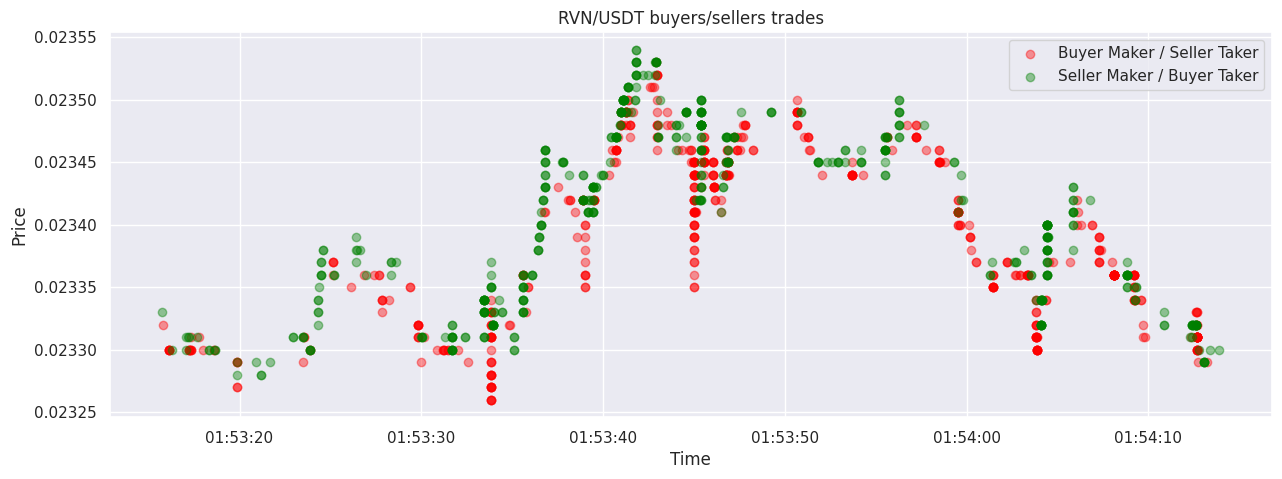
\includegraphics[width=\linewidth,height=0.6\textheight,keepaspectratio]{gfx/m3l3_notes_fig5_buyer_seller_scatter.png}
\par\smallskip{\small \textbf{Hình 3.5:} Biểu đồ phân tán giá các giao dịch RVN/USDT trong khoảng một phút, phân biệt bên mua tạo lập/bên bán nhận lệnh (đỏ) và bên bán tạo lập/bên mua nhận lệnh (xanh lá)}
\end{figure}

\textbf{Bài tập 3}

Trong Hình 3.5, ta thấy một đồ thị phóng to các giao dịch của bên mua và bên bán của RVN/USDT. Khoảng thời gian được chọn chính xác là 1 phút. Trong bài tập này, bạn phải tạo lại Hình 3.5 cho các khoảng thời gian khác nhau. Bạn có thể chọn các khoảng dài hơn và/hoặc các thời điểm khác nhau. Để có một hướng dẫn trong việc chọn các khoảng thời gian mà bạn \textbf{quan tâm}, bạn sẽ phải vẽ toàn bộ đồ thị giá của cặp RVN/USDT.

\textbf{Bài tập 4} \emph{(Tùy chọn)}

Dùng mã được cung cấp trong notebook này làm hướng dẫn, hãy tải dữ liệu tick về máy cục bộ để tiếp tục quy trình làm việc trên máy tính của riêng bạn. Sau đó, hãy thử dùng plotly hoặc bokeh (holoviews) để tạo các đồ thị tương tác cho phép bạn phóng to mà không phải cắt lát tập dữ liệu mỗi khi muốn tạo một đồ thị mới. Xem thư viện đồ thị do plotly cung cấp tại \url{https://plotly.com/python/}, và đảm bảo bạn hiểu sự khác biệt giữa đồ thị tương tác và đồ thị tĩnh.

\section{Dữ liệu Cấp 1 (Level 1, L1)}

Dữ liệu Level 1 (hay còn gọi là dữ liệu đỉnh sổ lệnh, top-of-book data, TOB) thường bao gồm các cột sau:

\begin{itemize}
  \item Symbol: mã định danh duy nhất của công cụ tài chính.
  \item Timestamp: thời điểm chính xác khi sự kiện được ghi nhận.
  \item Bid price: mức giá cao nhất mà một bên mua sẵn sàng trả.
  \item Ask price: mức giá thấp nhất mà một bên bán sẵn sàng chấp nhận.
  \item Ask volume (khối lượng chào bán): số đơn vị có sẵn tại mức giá chào bán.
  \item Bid Volume (khối lượng chào mua): số đơn vị có sẵn tại mức giá chào mua.
\end{itemize}

\begin{lstlisting}[language=Python,escapeinside={(*@}{@*)}]
# (*@Tải@*) (*@dữ@*) (*@liệu@*), (*@tập@*) (*@dữ@*) (*@liệu@*) (3) - AGLJ_J
columns = ['RIC', 'DateTimeL', 'Type', 'Price', 'Volume', 'L1 Bid', 'L1 Ask', 'Trade Sign']
aglj = pd.read_csv('AGLJ_J_04-Jan-2016_TO_10-May-2016_5days.csv', \
                   names = columns, skiprows = 1) # (*@Tải@*) (*@dữ@*) (*@liệu@*)
aglj.sort_values(by = 'DateTimeL', inplace = True)
aglj.head(5)
\end{lstlisting}

\begin{lstlisting}[escapeinside={(*@}{@*)}]
       RIC      DateTimeL    Type   Price  Volume  L1 Bid  L1 Ask  Trade Sign
0   AGLJ.J  736333.382013   Trade  6750.0   366.0     0.0     0.0         0.0
1   AGLJ.J  736333.382013   Quote     0.0     0.0     0.0  6800.0         0.0
2   AGLJ.J  736333.382015   Trade  6750.0   374.0     0.0     0.0         0.0
3   AGLJ.J  736333.382015   Quote     0.0     0.0     0.0  6800.0         0.0
4   AGLJ.J  736333.382015   Quote     0.0     0.0  6735.0  6800.0         0.0
\end{lstlisting}

Điều đầu tiên cần chú ý là cột \texttt{DateTimeL}. Đây là một định dạng khác mà bạn có thể gặp khi dùng dữ liệu tick, và nó biểu diễn một số \emph{ngày tuần tự (serial date)} thể hiện ngày và giờ. Cụ thể, nó đếm số ngày tính từ một ngày cho trước, gọi là \texttt{base\_date}. Trong trường hợp của chúng ta, \texttt{base\_date} là ngày 1 tháng 1 năm 0000. Ví dụ, 736333.382013 được hiểu là ngày thứ 736333 kể từ ngày 1 tháng 1 năm 0000. Phần thập phân biểu diễn phần của ngày. Trong ví dụ của chúng ta, ngày thứ 736333 là ngày 4 tháng 1 năm 2016, và phần 0.382013 tương ứng với 09:10:05.

Với sự trợ giúp của thư viện Python \texttt{datetime}, chúng ta sẽ chuyển ngày tuần tự thành dạng dễ đọc. Nhưng việc này không phải không có vấn đề! Lịch của thư viện \texttt{datetime} bắt đầu từ ngày 1 tháng 1 năm 0001, vì về mặt lịch sử không có năm 0000. Mặt khác, việc đánh chỉ số từ 0 được ưu tiên trong các tính toán khoa học. Sinh viên không cần đi sâu vào vấn đề này, nhưng đây là một ví dụ tốt về các cách ký hiệu khác nhau mà người ta gặp phải khi xử lý dữ liệu tick.

\begin{lstlisting}[language=Python,escapeinside={(*@}{@*)}]
from datetime import datetime, timedelta

def convert_serial_to_datetime(serial):
    # (*@Xác@*) (*@định@*) (*@ngày@*) (*@cơ@*) (*@sở@*) (*@là@*) (*@ngày@*) 1 (*@tháng@*) 1 (*@năm@*) 0001
    base_date = datetime(1, 1, 1)

    # (*@Tách@*) (*@ngày@*) (*@tuần@*) (*@tự@*) (*@thành@*) (*@số@*) (*@ngày@*) (*@và@*) (*@phần@*) (*@lẻ@*) (*@của@*) (*@ngày@*)
    days = int(serial)
    fractional_day = serial - days

    # (*@Điều@*) (*@chỉnh@*) (*@do@*) (*@không@*) (*@có@*) (*@năm@*) 0 (*@bằng@*) (*@cách@*) (*@trừ@*) (*@đi@*) 367 (*@ngày@*)
    adjusted_days = days - 367

    # (*@Tính@*) (*@ngày@*) (*@đích@*) (*@bằng@*) (*@cách@*) (*@cộng@*) (*@số@*) (*@ngày@*) (*@đã@*) (*@điều@*) (*@chỉnh@*) (*@và@*) (*@phần@*) (*@lẻ@*) (*@của@*) (*@ngày@*) ((*@quy@*) (*@đổi@*) (*@ra@*) (*@giây@*)) (*@vào@*) (*@ngày@*) (*@cơ@*) (*@sở@*)
    target_date = base_date + timedelta(days=adjusted_days) + timedelta(seconds=fractional_day * 86400)

    # (*@Trả@*) (*@về@*) (*@ngày@*) (*@đích@*) (*@ở@*) (*@định@*) (*@dạng@*) (*@dễ@*) (*@đọc@*)
    return target_date.strftime('%Y-%m-%d %H:%M:%S')

aglj['timestamp'] = aglj['DateTimeL'].apply(convert_serial_to_datetime) # (*@Chuyển@*) (*@ngày@*) (*@tuần@*) (*@tự@*) (*@thành@*) (*@ngày@*) (*@giờ@*) (*@dễ@*) (*@đọc@*)
aglj['timestamp'] = pd.to_datetime(aglj['timestamp']) # (*@Chuyển@*) (*@mốc@*) (*@thời@*) (*@gian@*) (*@thành@*) (*@đối@*) (*@tượng@*) (*@datetime@*)
aglj.set_index('timestamp', inplace=True) # (*@Đặt@*) (*@timestamp@*) (*@làm@*) (*@chỉ@*) (*@mục@*)
aglj.head(5)
\end{lstlisting}

\begin{lstlisting}[escapeinside={(*@}{@*)}]
                         RIC      DateTimeL    Type   Price  Volume  L1 Bid  \
timestamp                                                                     
2016-01-04 09:10:05   AGLJ.J  736333.382013   Trade  6750.0   366.0     0.0   
2016-01-04 09:10:05   AGLJ.J  736333.382013   Quote     0.0     0.0     0.0   
2016-01-04 09:10:06   AGLJ.J  736333.382015   Trade  6750.0   374.0     0.0   
2016-01-04 09:10:06   AGLJ.J  736333.382015   Quote     0.0     0.0     0.0   
2016-01-04 09:10:06   AGLJ.J  736333.382015   Quote     0.0     0.0  6735.0   

                     L1 Ask  Trade Sign  
timestamp                                
2016-01-04 09:10:05     0.0         0.0  
2016-01-04 09:10:05  6800.0         0.0  
2016-01-04 09:10:06     0.0         0.0  
2016-01-04 09:10:06  6800.0         0.0  
2016-01-04 09:10:06  6800.0         0.0  
\end{lstlisting}

Bây giờ hãy áp dụng một số bộ lọc làm sạch:

Trước khi có thể phân tích hiệu quả dữ liệu tài chính tần suất cao, điều thiết yếu là làm sạch và tiền xử lý tập dữ liệu. Quá trình làm sạch này giúp loại bỏ các bản ghi sai sót và điều chỉnh một số hiệu ứng vi cấu trúc thị trường, đảm bảo rằng các phân tích sau đó dựa trên dữ liệu chính xác và có ý nghĩa.

Trước hết, chúng ta loại bỏ các bản ghi có giá, báo giá hoặc khối lượng bằng không hoặc âm. Đây nhiều khả năng là lỗi dữ liệu, vì giá và khối lượng trong các thị trường tài chính luôn phải dương. Các chênh lệch âm (negative spread), tức khi giá chào mua vượt giá chào bán, cũng bị loại bỏ vì chúng biểu diễn các điều kiện thị trường bất khả thi trong hoàn cảnh bình thường.

Tiếp theo, chúng ta giải quyết vấn đề giao dịch bị chia nhỏ. Trong giao dịch tần suất cao, một lệnh lớn duy nhất có thể được thực thi thành nhiều giao dịch nhỏ hơn tại cùng một mốc thời gian. Điều này có thể dẫn đến việc biểu diễn quá mức một số mức giá và có khả năng làm lệch phân tích của chúng ta. Để giảm thiểu điều này, chúng ta gộp các giao dịch xảy ra tại cùng một mốc thời gian, cộng khối lượng của chúng và tính giá trung bình theo khối lượng (VWAP). Cách tiếp cận này bảo toàn thông tin giao dịch tổng thể đồng thời tránh làm phồng giả tạo số lượng giao dịch.
Tương tự, chúng ta xử lý các báo giá trong cùng một giây bằng cách chỉ giữ lại báo giá cuối cùng cho mỗi mốc thời gian. Lý do là trong một thị trường biến động nhanh, báo giá gần nhất thường là báo giá liên quan nhất cho phân tích.

\begin{lstlisting}[language=Python,escapeinside={(*@}{@*)}]
# (*@Xóa@*) (*@các@*) (*@bản@*) (*@ghi@*) (*@có@*) (*@giá@*) (*@báo@*) (*@giá@*) (*@hoặc@*) (*@giá@*) (*@giao@*) (*@dịch@*) (*@bằng@*) (*@không@*) (*@hoặc@*) (*@âm@*)
prices = aglj[aglj['Type'] == ' Trade']['Price']
quotes = aglj[aglj['Type'] == ' Quote'][['L1 Bid', 'L1 Ask']]
print("Number of entries with a transaction price equal to zero or negative: ", (prices <= 0).sum())
print("Number of entries with negative or zero volume: ", (aglj[aglj['Type'] == ' Trade']['Volume'] <= 0).sum())
print("Number of entries with a quote equal to zero or negative: ", (quotes <= 0).sum().sum())
index_to_drop_quotes = quotes[quotes['L1 Ask'] <= 0].index.union(quotes[quotes['L1 Bid'] <= 0].index)
aglj.drop(index=index_to_drop_quotes, inplace=True)

# (*@Xóa@*) (*@các@*) (*@bản@*) (*@ghi@*) (*@có@*) (*@chênh@*) (*@lệch@*) (*@âm@*)
spreads = aglj[aglj['Type'] == ' Quote']['L1 Ask'] - aglj[aglj['Type'] == ' Quote']['L1 Bid']
index_to_drop_spreads = spreads[spreads < 0].index
print("Number of entries with a negative spread: ", len(index_to_drop_spreads))
aglj.drop(index=index_to_drop_spreads, inplace=True)

# (*@Xử@*) (*@lý@*) (*@các@*) (*@giao@*) (*@dịch@*) (*@bị@*) (*@chia@*) (*@nhỏ@*)
dataset_on_trades = aglj[aglj['Type'] == ' Trade'].copy()

grouped_trades = dataset_on_trades.groupby('DateTimeL')
unique_trades = pd.DataFrame({
    'DateTimeL': grouped_trades['DateTimeL'].first(),
    'Volume': grouped_trades['Volume'].sum(),
    'Price': (dataset_on_trades['Price'] * dataset_on_trades['Volume']).groupby(dataset_on_trades['DateTimeL']).sum() / grouped_trades['Volume'].sum(),
    'L1 Bid': 0.0,  # (*@Giữ@*) (*@cấu@*) (*@trúc@*) (*@nhất@*) (*@quán@*)
    'L1 Ask': 0.0,  # (*@Giữ@*) (*@cấu@*) (*@trúc@*) (*@nhất@*) (*@quán@*)
    'Type': ' Trade'
})

# (*@Lấy@*) (*@dấu@*) (*@giao@*) (*@dịch@*) (*@cuối@*) (*@cùng@*) (*@cho@*) (*@mỗi@*) (*@mốc@*) (*@thời@*) (*@gian@*) (*@đã@*) (*@nhóm@*)
trade_signs = dataset_on_trades.groupby('DateTimeL')['Trade Sign'].last()
unique_trades['Trade Sign'] = unique_trades['DateTimeL'].map(trade_signs)

# (*@Xử@*) (*@lý@*) (*@các@*) (*@báo@*) (*@giá@*) (*@trong@*) (*@cùng@*) (*@một@*) (*@giây@*)
dataset_on_quotes = aglj[aglj['Type'] == ' Quote'].copy()

unique_quotes = pd.DataFrame({
    'DateTimeL': dataset_on_quotes.groupby('DateTimeL')['DateTimeL'].last(),
    'Volume': 0.0,  # (*@Giữ@*) (*@cấu@*) (*@trúc@*) (*@nhất@*) (*@quán@*)
    'Price': 0.0,   # (*@Giữ@*) (*@cấu@*) (*@trúc@*) (*@nhất@*) (*@quán@*)
    'L1 Bid': dataset_on_quotes.groupby('DateTimeL')['L1 Bid'].last(),
    'L1 Ask': dataset_on_quotes.groupby('DateTimeL')['L1 Ask'].last(),
    'Type': ' Quote',
    'Trade Sign': 0.0  # (*@hoặc@*) np.nan (*@nếu@*) (*@bạn@*) (*@muốn@*)
})

# (*@Dùng@*) (*@concat@*) (*@thay@*) (*@vì@*) (*@merge@*) ((*@vì@*) (*@ta@*) (*@giữ@*) (*@tất@*) (*@cả@*) (*@các@*) (*@cột@*))
aggr_dataset_2 = pd.concat([unique_trades, unique_quotes], ignore_index=True)

# (*@Sắp@*) (*@xếp@*) (*@theo@*) DateTimeL
aggr_dataset_2 = aggr_dataset_2.sort_values('DateTimeL').reset_index(drop=True)

# (*@Đặt@*) (*@chỉ@*) (*@mục@*) (*@và@*) (*@chuyển@*) (*@sang@*) (*@datetime@*)
aggr_dataset_2.set_index('DateTimeL', inplace=True)
aggr_dataset_2.index = pd.to_datetime(aggr_dataset_2.index.map(convert_serial_to_datetime))
aggr_dataset_2.index.name = 'DateTimeL'

aggr_dataset_2.head(5)
\end{lstlisting}

\begin{lstlisting}[escapeinside={(*@}{@*)}]
Number of entries with a transaction price equal to zero or negative:  0
Number of entries with negative or zero volume:  0
Number of entries with a quote equal to zero or negative:  16
Number of entries with a negative spread:  32
\end{lstlisting}

\begin{lstlisting}[escapeinside={(*@}{@*)}]
                     Volume  Price  L1 Bid  L1 Ask    Type  Trade Sign
DateTimeL                                                             
2016-01-04 09:10:20     0.0    0.0  6751.0  6800.0   Quote         0.0
2016-01-04 09:10:20     0.0    0.0  6751.0  6800.0   Quote         0.0
2016-01-04 09:10:21     0.0    0.0  6755.0  6800.0   Quote         0.0
2016-01-04 09:10:21     0.0    0.0  6757.0  6800.0   Quote         0.0
2016-01-04 09:10:42     0.0    0.0  6759.0  6800.0   Quote         0.0
\end{lstlisting}

\begin{lstlisting}[language=Python,escapeinside={(*@}{@*)}]
# (*@Số@*) (*@dòng@*) (*@giảm@*) (*@đáng@*) (*@kể@*)
print(f"The filtered dataset `aggr_dataset_2` has {len(aggr_dataset_2)} entries, while the `aglj` dataset had {len(aglj)}.")
\end{lstlisting}

\begin{lstlisting}[escapeinside={(*@}{@*)}]
The filtered dataset `aggr_dataset_2` has 109579 entries, while the `aglj` dataset had 138477.
\end{lstlisting}

\section{Mất cân bằng Dòng lệnh (Order Flow Imbalance, OFI)}

Mất cân bằng dòng lệnh (Order Flow Imbalance, OFI) là một khái niệm quan trọng trong phân tích dữ liệu tần suất cao, cung cấp hiểu biết về áp lực mua và bán trên thị trường. Nó đo dòng lệnh ròng bằng cách xét đến cả hướng và kích thước của các giao dịch. Chúng ta sẽ tính dạng OFI đơn giản nhất bằng cách nhân cột \texttt{Trade Sign} (dấu dương cho các giao dịch do bên mua khởi tạo và dấu âm cho các giao dịch do bên bán khởi tạo) với khối lượng giao dịch tương ứng. Theo thời gian, tổng lũy kế của các khối lượng có dấu này cho ta OFI. OFI dương cho thấy áp lực mua ròng, còn OFI âm gợi ý áp lực bán ròng. Bằng cách phân tích OFI, ta có thể thu được những hiểu biết có giá trị về các biến động giá ngắn hạn, động lực thanh khoản và các xu hướng giá tiềm năng trong tương lai (như lý thuyết gợi ý).

\begin{lstlisting}[language=Python,escapeinside={(*@}{@*)}]
# (*@Hình@*) 3.6
signed_volume = aggr_dataset_2[aggr_dataset_2['Type'] == ' Trade']['Volume'] * aggr_dataset_2[aggr_dataset_2['Type'] == ' Trade']['Trade Sign'] # (*@Tính@*) OFI
ofi = signed_volume.cumsum() # (*@Tính@*) (*@tổng@*) (*@lũy@*) (*@kế@*) (*@của@*) OFI
prices = aggr_dataset_2[aggr_dataset_2['Type'] == ' Trade']['Price'] # (*@Lấy@*) (*@giá@*)

fig, ax = plt.subplots(figsize=(15, 5))
ax.plot(np.arange(len(ofi)), ofi, label = 'OFI', color = 'red', alpha = 0.5) # (*@Vẽ@*) OFI
ax.set_ylabel('OFI')
ax.set_xlabel('Number of Ticks')
ax.set_title('Order Flow Imbalance (OFI) for AGLJ_J')
ax.set_ylim(-100000, 2000000)
ax.legend(loc = 'lower right')

ax2 = ax.twinx()
ax2.plot(np.arange(len(prices)), prices, color='blue', label='Price', alpha=0.7)
ax2.set_ylabel('Price')
ax2.legend()
ax2.set_ylim(4000, 7000)
plt.show()

print("\n\nThe Pearson correlation between the price and OFI is: ", np.corrcoef(prices, ofi)[0, 1]) # (*@Tính@*) (*@tương@*) (*@quan@*) (*@Pearson@*) (*@giữa@*) (*@giá@*) (*@và@*) OFI
\end{lstlisting}

\begin{figure}[H]
\centering
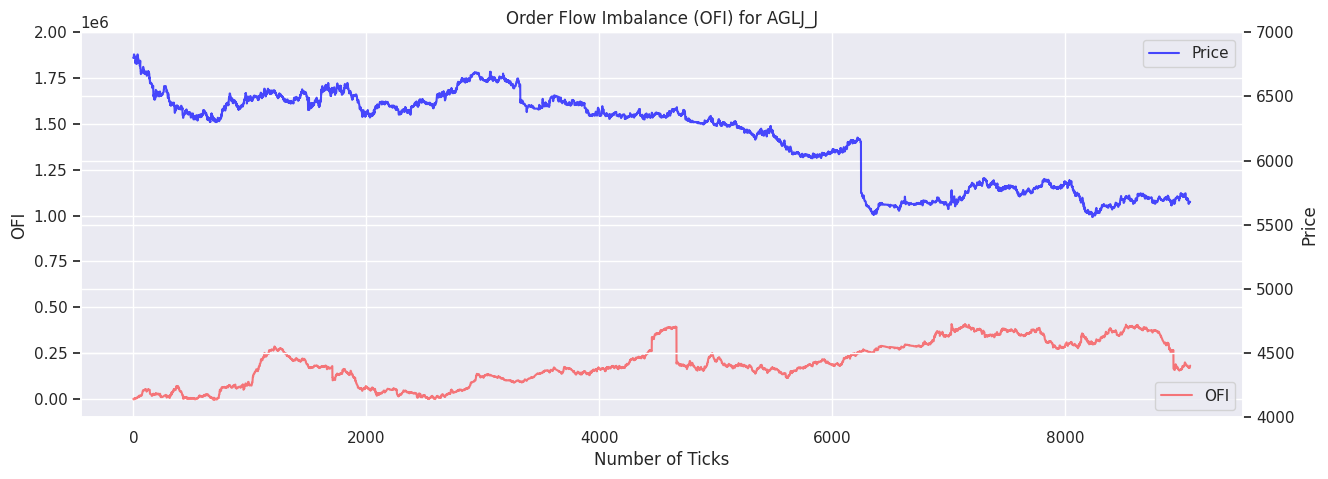
\includegraphics[width=\linewidth,height=0.6\textheight,keepaspectratio]{gfx/m3l3_notes_fig6_order_flow_imbalance.png}
\par\smallskip{\small \textbf{Hình 3.6:} Mất cân bằng dòng lệnh (OFI) lũy kế và giá của AGLJ\_J theo số tick}
\end{figure}

\begin{lstlisting}[escapeinside={(*@}{@*)}]


The Pearson correlation between the price and OFI is:  -0.7586082958132966
\end{lstlisting}

\textbf{Bài tập 5}

Hãy import thư viện \texttt{scipy} và tính tương quan Spearman và Kendall giữa giá và OFI. Bạn thấy gì? Kết quả đó có như bạn kỳ vọng không?

Kết quả trên có phần phản trực giác và rất phổ biến trong thực tế. Nó nhấn mạnh tầm quan trọng của phân tích thực nghiệm với dữ liệu thế giới thực thay vì chỉ dựa vào các kỳ vọng lý thuyết.

Như ta thấy, giá của AGLJ trong năm ngày này có độ dốc đi xuống. Trong một số trường hợp, giá có độ dốc đi lên ngắn hạn, nhưng xu hướng chung là rõ ràng. Với giá như vậy, kỳ vọng của chúng ta (dựa trên lý thuyết và trực giác) sẽ là OFI cũng có độ dốc đi xuống. Nhưng điều này hầu như không xảy ra vì OFI dường như gần như hoàn toàn không nhất quán với giá. Khối lượng mua (theo định nghĩa trong notebook này) đang tăng, nghĩa là có nhiều bên mua (bên nhận lệnh) hơn bên bán, trong khi đồng thời giá lại đang giảm.

Có thể có nhiều lý do cho hiện tượng này, và chúng có thể rất khác nếu dữ liệu được lấy từ một sàn giao dịch khác hoặc cho một khoảng thời gian khác:

\begin{itemize}
  \item Hành vi của nhà tạo lập thị trường/nhà giao dịch: Các nhà tạo lập thị trường hoặc các nhà giao dịch lớn có thể đang cung cấp thanh khoản khi giá giảm, hấp thụ các lệnh bán. Điều này sẽ hiện ra như OFI dương (vì họ đang mua) ngay cả khi giá tiếp tục giảm.
  \item Các giao dịch lớn: Một vài lệnh bán lớn có thể có trọng lượng lớn hơn nhiều lệnh mua nhỏ.
  \item Hiệu ứng vi cấu trúc thị trường: Trong một số cấu trúc thị trường, các lệnh bán lớn có thể kích hoạt một chuỗi các lệnh mua nhỏ hơn khi chúng được khớp, điều này có thể dẫn đến mẫu hình này.
  \item Cân nhắc về khung thời gian: Mối quan hệ giữa OFI và giá có thể khác nhau ở các thang thời gian khác nhau. Những gì ta thấy có thể là một hiệu ứng ngắn hạn có thể đảo chiều trong các giai đoạn dài hơn.
\end{itemize}

\textbf{Bài tập 6}

Chúng ta cố ý đưa ra một định nghĩa cho khối lượng mua và bán: Khối lượng mua/bán là khối lượng của các giao dịch được khởi tạo bởi bên mua/bên bán (với tư cách bên nhận lệnh). Nhưng bây giờ chúng ta phải nghĩ về khối lượng mua và bán từ góc nhìn ý định của nhà giao dịch, tức là khối lượng mua và bán thực sự.

Gợi ý: Nếu một nhà giao dịch muốn mua, họ có thể đặt một lệnh thị trường hoặc một lệnh giới hạn.

Hãy khởi xướng một cuộc thảo luận trên diễn đàn với các ý tưởng của bạn.

\textbf{Bài tập 7}

Chúng ta đã quan sát thấy một kết quả phản trực giác liên quan đến OFI của tập dữ liệu (3): giá giảm trong khi OFI tăng. Bây giờ hãy tính OFI cho tập dữ liệu (2) và vẽ nó cùng với giá trên cùng một đồ thị (hai trục $y$). Bạn thấy gì?

Bây giờ hãy đưa ra các ý tưởng để vẽ giá chào mua và giá chào bán tốt nhất cùng với giá của AGLJ: chúng ta sẽ dùng hàm bậc thang (step) cho các mức báo giá và biểu đồ phân tán (scatter) cho giá.

\begin{lstlisting}[language=Python,escapeinside={(*@}{@*)}]
# (*@Hình@*) 3.7

zoomed_in_quotes_price = aggr_dataset_2.loc['2016-01-04'].iloc[15000:17000, :] # (*@Cắt@*) (*@lát@*) (*@dữ@*) (*@liệu@*)

fig, ax = plt.subplots(figsize=(15, 5))

ax.scatter(x = zoomed_in_quotes_price[(zoomed_in_quotes_price['Type'] == ' Trade') & (zoomed_in_quotes_price['Trade Sign'] == 1)].index, \
              y = zoomed_in_quotes_price[(zoomed_in_quotes_price['Type'] == ' Trade') & (zoomed_in_quotes_price['Trade Sign'] == 1)]['Price'], color='green', \
                label='Buyer initiated Trades', alpha = 0.7, s = 40) # (*@Vẽ@*) (*@các@*) (*@giao@*) (*@dịch@*)
ax.scatter(x = zoomed_in_quotes_price[(zoomed_in_quotes_price['Type'] == ' Trade') & (zoomed_in_quotes_price['Trade Sign'] == -1)].index, \
              y = zoomed_in_quotes_price[(zoomed_in_quotes_price['Type'] == ' Trade') & (zoomed_in_quotes_price['Trade Sign'] == -1)]['Price'], color='red', \
                label='Seller initiated Trades', alpha = 0.7, s = 40) # (*@Vẽ@*) (*@các@*) (*@giao@*) (*@dịch@*)
ax.step(zoomed_in_quotes_price[zoomed_in_quotes_price['Type'] == ' Quote'].index, \
                zoomed_in_quotes_price[zoomed_in_quotes_price['Type'] == ' Quote']['L1 Bid'], color='green', \
                    label='L1 Bid', alpha = 0.8, where = 'post') # (*@Vẽ@*) L1 Bid
ax.step(zoomed_in_quotes_price[zoomed_in_quotes_price['Type'] == ' Quote'].index, \
                zoomed_in_quotes_price[zoomed_in_quotes_price['Type'] == ' Quote']['L1 Ask'], color='red', \
                    label='L1 Ask', alpha = 0.4, where = 'post') # (*@Vẽ@*) L1 Ask

ax.set_title("AGLJ_J trades and L1 Bid/Ask")
ax.set_xlabel("Time")
ax.set_ylabel("Price")
ax.legend()
plt.show()
\end{lstlisting}

% [Nguyên bản không có ảnh kết quả đã lưu cho ô mã Hình 3.7]

\textbf{Bài tập 8}

Trong Hình 3.7, bạn có thể thấy đồ thị các báo giá tốt nhất được vẽ cùng với giá. Hãy làm như sau:
\begin{itemize}
  \item Hãy chắc chắn bạn có thể giải thích đối số \texttt{where = 'post'} bên trong hàm vẽ step.
  \item Bằng cách xem tài liệu của \texttt{matplotlib}, hãy cải tiến đồ thị trên bằng cách điều chỉnh kích thước của marker scatter theo kích thước giao dịch. Cụ thể, nếu giao dịch A lớn hơn giao dịch B thì marker A phải lớn hơn marker B. Bạn có thể chọn một ngày khác và một lát cắt khác của tập dữ liệu. Hãy dán kết quả của bạn lên diễn đàn.
\end{itemize}

\section{Lấy mẫu lại (Resampling)}

Ở mục cuối này, chúng ta sẽ tạo ra các thanh thời gian (time bar) mà ai cũng quen thuộc. Vì lý do này, chúng ta sẽ dùng phương thức \texttt{resample} hoạt động rất tốt với chỉ mục datetime. Chúng ta sẽ tạo các tập dữ liệu cho nhiều khung thời gian và sẽ minh họa cách một số thống kê thay đổi khi khung thời gian lớn dần. Tập dữ liệu chúng ta chọn sẽ là tập dữ liệu (2): rvn\_usdt.

\begin{lstlisting}[language=Python,escapeinside={(*@}{@*)}]
rvn_usdt
\end{lstlisting}

\begin{lstlisting}[language=Python,escapeinside={(*@}{@*)}]
#(*@Tạo@*) (*@hàm@*) (*@resample@*)
def calculate_statistics(df: pd.DataFrame, freq: str) -> dict:
    """
    (*@Tính@*) (*@các@*) (*@thống@*) (*@kê@*) (*@cho@*) (*@một@*) (*@khung@*) (*@thời@*) (*@gian@*) (*@đơn@*) (*@lẻ@*) (*@mà@*) (*@không@*) (*@lưu@*) (*@dữ@*) (*@liệu@*) (*@trung@*) (*@gian@*).
    """
    # (*@Chỉ@*) (*@lấy@*) (*@mẫu@*) (*@lại@*) (*@giá@*) (*@đóng@*) (*@cửa@*) ((*@không@*) (*@phải@*) OHLC)
    resampled_close = df['price'].resample(freq, label='right').last()
    
    # (*@Tính@*) (*@lợi@*) (*@suất@*) (*@log@*)
    log_returns = np.log(resampled_close / resampled_close.shift(1)).dropna()
    
    # (*@Tính@*) (*@và@*) (*@trả@*) (*@về@*) (*@các@*) (*@thống@*) (*@kê@*) (*@ngay@*) (*@lập@*) (*@tức@*)
    stats = {
        'mean': log_returns.mean(),
        'std': log_returns.std(),
        'skewness': log_returns.skew(),
        'kurt': log_returns.kurt()
    }
    
    # (*@Bộ@*) (*@nhớ@*) (*@được@*) (*@giải@*) (*@phóng@*) (*@tự@*) (*@động@*) (*@khi@*) (*@hàm@*) (*@trả@*) (*@về@*)
    return stats

# (*@Xử@*) (*@lý@*) (*@từng@*) (*@khung@*) (*@thời@*) (*@gian@*) (*@một@*)
timeframes = ['1min', '2min', '5min', '10min', '15min', '30min', '1h', '2h', '4h', '8h', '12h', '1D', '2D', '5D']
statistics = {}

for timeframe in timeframes:
    statistics[timeframe] = calculate_statistics(rvn_usdt, timeframe)
\end{lstlisting}

\textbf{Bài tập 9}

Hãy giải thích đối số \texttt{label = right}. Hãy thảo luận các ý tưởng của bạn trên diễn đàn. Ngoài ra, hãy tìm một thư viện phù hợp để vẽ các ``nến'' (candle) cùng với khối lượng.

\begin{lstlisting}[language=Python,escapeinside={(*@}{@*)}]
#(*@Hình@*) 3.8
pd.DataFrame(statistics).T.plot(subplots = True, figsize = (15, 5), layout = (2, 2), title = 'RVN/USDT Price Statistics', alpha = 0.7) # (*@Vẽ@*) (*@các@*) (*@thống@*) (*@kê@*)
plt.show()
\end{lstlisting}

% [Nguyên bản không có ảnh kết quả đã lưu cho ô mã Hình 3.8]

Các kết quả trên phần nào là điều có thể dự đoán và cho ta thấy những tính chất mà ta mất đi hoặc thu được khi tổng hợp dữ liệu tần suất cao.

\begin{itemize}
  \item Lợi suất trung bình gần bằng 0 ở các khung thời gian nhỏ. Vì mỗi giao dịch tương ứng với các bước giá nhỏ, nên tự nhiên là các thay đổi giá ở khung thời gian nhỏ không thể tích lũy để cho thấy một giá trị trung bình khác không.
  \begin{enumerate}
    \item Nhiễu vi cấu trúc thị trường (Microstructure Noise): Ở tần suất rất cao, lợi suất chịu ảnh hưởng nặng nề của các hiệu ứng vi cấu trúc thị trường như hiện tượng nảy giá chào mua-chào bán (bid-ask bounce), có thể che lấp bất kỳ xu hướng giá thực sự nào trong các khoảng ngắn.
    \item Tính chất martingale (Martingale Property): Trong một thị trường công bằng, các quá trình giá thường được mô hình hóa như martingale, trong đó giá kỳ vọng trong tương lai, cho trước mọi thông tin quá khứ, chính là giá hiện tại. Điều này hàm ý rằng lợi suất kỳ vọng ngắn hạn phải bằng không.
  \end{enumerate}
  \item Độ lệch chuẩn (Standard Deviation): Việc độ lệch chuẩn tăng theo khung thời gian lớn hơn phù hợp với các tính chất của chuyển động Brown (Brownian motion) (xem thêm trong môn Định giá Phái sinh), vốn được dùng để mô hình hóa các quá trình giá. Theo các giả định của chuyển động Brown, phương sai tăng tuyến tính theo thời gian, do đó độ lệch chuẩn tăng theo căn bậc hai của thời gian.
  \item Độ dốc đi lên nhẹ của độ lệch (skewness) khi khung thời gian lớn dần có thể cho thấy rằng các biến động giá dương có xu hướng lớn hơn các biến động giá âm trong các giai đoạn dài hơn.
  \item Quan trọng hơn, độ nhọn (kurtosis) cao ở các khung thời gian nhỏ phản ánh bản chất nhọn (leptokurtic) của lợi suất tần suất cao. Cụ thể hơn:
  \begin{enumerate}
    \item Đuôi béo (Fat Tails): Các sự kiện cực đoan xảy ra phổ biến trong phân phối nhọn, phổ biến hơn so với phân phối chuẩn.
    \item Khi ta tổng hợp lên các khung thời gian lớn hơn, định lý giới hạn trung tâm phát huy tác dụng và phân phối lợi suất tiến gần đến phân phối chuẩn. Tuy nhiên, ở các khung thời gian lớn hơn, lợi suất vẫn chưa đạt tới phân phối chuẩn.
  \end{enumerate}
\end{itemize}

\textbf{Bài tập 10}

Hãy tạo các thanh thời gian cho cặp rvn\_usdt như ở trên nhưng bây giờ thêm hai cột nữa:
\begin{itemize}
  \item Một cột tên \texttt{buying\_volume} gồm khối lượng tổng hợp của các giao dịch thuộc \texttt{is\_buyer\_maker = False}
  \item Một cột tên \texttt{selling\_volume} gồm khối lượng tổng hợp của các giao dịch thuộc \texttt{is\_buyer\_maker = True}
\end{itemize}

\textbf{Bài tập 11}

Khi giải thích các thống kê của Hình 3.8, chúng ta đã dùng định lý giới hạn trung tâm để lập luận cho sự hội tụ của phân phối lợi suất về phân phối chuẩn. Nhưng thực ra chúng ta không hề tổng hợp các lợi suất. Thay vào đó, chúng ta dùng cột \texttt{close} của mỗi khung thời gian để tính độ nhọn. Lập luận đó có được dùng đúng hay không? Vì sao? Hãy làm như trên nhưng thay vì giá \texttt{close} của mỗi khung thời gian, hãy tính \texttt{sum()} của các lợi suất log. Điều này có thay đổi gì không?

\section{Kết luận}

Bài học này đã cung cấp phần giới thiệu về dữ liệu tick, các đặc điểm của nó và tầm quan trọng của nó trong các thị trường tài chính. Chúng ta đã khám phá cấu trúc của dữ liệu giao dịch từng tick và dữ liệu Level 1, minh họa cách xử lý, làm sạch và vẽ các tập dữ liệu tần suất cao này.

Những điểm chính cần ghi nhớ gồm:

\begin{enumerate}
  \item Độ chi tiết của dữ liệu tick mang lại những hiểu biết về vi cấu trúc thị trường mà không thể thấy được trong dữ liệu tần suất thấp hơn.
  \item Làm sạch là một bước tiền xử lý thiết yếu, cần bao gồm việc xử lý các giao dịch bị chia nhỏ và các báo giá trong cùng một giây (cùng nhiều vấn đề khác).
  \item Mất cân bằng dòng lệnh (OFI) có thể cung cấp những hiểu biết có giá trị về động lực thị trường ngắn hạn, nhưng việc diễn giải nó đòi hỏi cân nhắc cẩn thận bối cảnh thị trường và có thể gây hiểu lầm.
  \item Lấy mẫu lại dữ liệu tick sang nhiều khung thời gian cho thấy các tính chất thống kê của lợi suất thay đổi ra sao theo sự tổng hợp thời gian, làm nổi bật sự đánh đổi giữa độ chi tiết và nhiễu.
  \item Làm việc với dữ liệu tick đặt ra những thách thức riêng, bao gồm khối lượng dữ liệu, các yêu cầu làm sạch, và nhu cầu về các kỹ thuật phân tích chuyên biệt.
\end{enumerate}

\textbf{Tài liệu tham khảo}

\begin{itemize}
  \item Gebbie, Tim, and Edward Nonyane. ``TRTH JSE AGLJ.J Intraday Transaction Test Data.'' Mendeley Data, V2, 2019.
  \item Harris, Larry. \emph{Trading and Exchanges: Market Microstructure for Practitioners}. Oxford University Press, 2003.
  \item Hautsch, Nikolaus. \emph{Econometrics of Financial High-Frequency Data}. Springer Science \& Business Media, 2011.
\end{itemize}
